\subsection*{Social Learning in Networks}

We adapt the model in \cite{brandl2024}. Specifically, we let $N = \{1, \ldots, n\}$ be the set of agents, and $T = \{1, 2, \ldots, t \}$ be the finite set of periods. In each period, each agent chooses an action $a$ from the same finite set of actions $A$. The finite set of states of the world is $\Omega$, where the true state $\omega \in \Omega$ is a random variable with full support distribution over $\Omega$. Agents share the same utility function $u : A \times \Omega \to \mathbb{R}$ that depends on their own action and the state of the world, where $a_\theta$ denotes the unique optimal (correct) action in that state. It's also assumed that $a_\theta \neq a_{\theta'}$ for any two distinct states $\theta, \theta' \in \Omega$. In each period $t \in T$, each agent $i$ privately observes a signal $s_t^i$ from a set of signals $S$. Conditional on each state $\theta$, $s_t^i$ has distribution $\mu_\theta \in \Delta(S)$, and signals are independent across agents and periods. Observing the signal realization $s \in S$ changes the log-likelihood ratio of the observing agent between the states $\theta$ and $\theta'$ by,
\[
\ell_{\theta, \theta'}(s) = \log \frac{d\mu_\theta(s)}{d\mu_{\theta'}(s)}.
\]
Each agent $i$ also observes the actions of her neighbors $N^i \subset N$, thus the information available to Agent $i$ in period $t$ before choosing an action is the collection of information sets $\mathcal{I}^i_{\leq t} = S^t \times A^{|N^i| \times (t-1)}$. It's said that Agent $i$ makes a mistake in period $t$ if $a_t^i \neq a_\omega$, and that $i$ learns at rate $r$ if,
\[
r = \liminf_{t \to \infty} -\frac{1}{t} \log P(a_t^i \neq a_\omega).
\]
Theorem 1 states that for any number of agents and any strategy profile, there exists an agent $i$ such that,
\[r^i \leq r_{bdd} = \min_{\theta \neq \theta'}\{E_\theta[\ell_{\theta,\theta'}] + E_{\theta'}[\ell_{\theta',\theta}]\}.\]


\subsection*{Partially Observable Markov Games}
Following the MARL literature, we model the social learning framework as a partially observable Markov game defined by the tuple,
\[(N, \Psi, A, \{O_i\}_{i \in N}, \Gamma, R, \gamma)\]
where,
\begin{itemize}
\item $N$ is the set of agents,
\item $\Psi $ is the Markov state space, with individual element $\psi$,
\item $A$ is the shared action space for all agents, with individual element $a$,
\item $O_i$ is the observation space for agent $i$, with individual element $o_i$,
\item $\Gamma : \Psi \times A^n \times \Psi \to [0,1]$ is the transition function,
\item $R: A \times \Psi \to \mathbb{R}$ is the shared reward function for all agents,
\item $\gamma \in [0,1)$ is the discount factor.
\end{itemize}

\subsubsection*{Markov States, Signals \& Actions}
For simplicity, we let $\Omega = \{\theta_1, \ldots, \theta_k\}$ be the set of possible states of the world; $S = \{s_k : \theta_k \in \Omega\}$ be the signal space, with $s_k$ being the signal for state $\theta_k$ and $A = \{a_k : \theta_k \in \Omega\}$ be the action space, with $a_k$ being the optimal action for state $\theta_k$. We can then define the Markov state space as 
\begin{equation*}
    \Psi = \{\omega\} \times S \times A^n
\end{equation*}
which accounts for the true state of the world, current period signal and current period actions. We leave the tracking of signal and action histories to the Recurrent Neural Networks (RNNs), thereby avoiding exponentially increasing Markov state space formulations.

\subsubsection*{Observations}
The observation for each agent $i$ at time $t$ is,
\begin{equation*}
o^i_t = (s^i_t, \bm{a_t}) \in O_i,
\end{equation*}
where $O_i = S \times A^n$ and $\bm{a_t} = \{a_t^1, \ldots, a_t^n\}$ is the action profile at period $t$.

\subsubsection*{Transitions}
The stochastic components of the Markov state transitions are the signal realizations and the actions taken by the agents. Formally, for state 
$\psi_t = (\omega, (s^i_t)_{i \in N}, \bm{a_t})$ and next state ${}\psi_{t+1} = (\omega, (s^i_{t+1})_{i \in N}, \bm{a_{t+1}} )$, the transition function can be written as,
\begin{equation*}
    \Gamma(\psi_{t+1}|\psi_t) = \prod_{i \in N} \mu_{\omega}(s^i_{t+1}) \prod_{i \in N} \sigma_t^i(\mathcal{I}^i_{\leq t})(a^i_{t+1})
\end{equation*}
where $\sigma_t^i$ is the \textit{policy} or \textit{strategy} of agent $i$ at period $t$. There are two important points to consider here. First, in this formulation, we condition the policies on action and signal histories that are not part of the Markov state space. The fact that we can still use this information to compute the policies stems from the technology of RNNs that allows for a memory buffer from past observations, without explicitly storing the observations themselves. Second, diverging from the original paper, we allow for policies to be time-dependent, which corresponds to the learning process of the RL agents.
\subsubsection*{Rewards}
The reward functions are identical across agents with $R_i(a, \psi)=R(a,\psi), \: \forall i \in N$. The true reward is the flow payoff $u(a^i_t, \omega)$, where $u: A \times \Omega \rightarrow \mathbb{R}$ is known but its realizations are not observed. Lacking this observation, we follow Huang et al. (2024) and construct an observed payoff function $v(a, s)$ with the property that, 
\[\mathbb{E}_{s \sim \mu^{\theta}}[v(a, s)] = u(a, \theta), \quad \forall \theta \in \Omega.\] Setting $u(a, \omega) = \mathbf{1}_{\{a=a^{\omega}\}}$ the problem of constructing such a function amounts to solving a system of $|\Omega|$ linear equations for each action.
More precisely, let $\bm{\mu}$ be an $k \times k$ matrix representing the signal distributions, where the entry $\mu^{\theta}(s)$ denotes the probability of observing signal $s$ in state $\theta$. We assume $\mu^{\theta}(s_{\theta}) > \mu^{\theta}(s)$, $\forall s \in S$, $\theta \in \Omega$, which implies that signal distributions are linearly independent across states and $\bm{\mu}$ is invertible. Similarly, for each action $a \in A$, define the \textit{utility vector} $\bm{u}_a \in \mathbb{R}^k$ as,
\begin{equation*}
    \bm{u}_a = \begin{bmatrix} u(a, \theta_1) \\ u(a, \theta_2) \\ \vdots \\ u(a, \theta_k) \end{bmatrix}.
\end{equation*}
The vector of observable reward functions $\bm{v}_a \in \mathbb{R}^n$ for action $a$ is the unique solution to the linear system as in,
\begin{align*}
    \bm{\mu} \bm{v}_a &= \bm{u}_a, \\
    \bm{v}_a &= \bm{\mu}^{-1} \bm{u}_a.
\end{align*}
Hence, the reward $v(a, s_j)$ for choosing action $a$ when observing signal $s_j$ is,
\begin{equation*}
    v(a, s_j) = \sum_{l=1}^k \left( \bm{\mu}^{-1} \right)_{jl} u(a, \theta_l),
\end{equation*}
where $\left( \bm{\mu}^{-1} \right)_{jl}$ denotes the $(j, l)$-th element of $\bm{\mu}^{-1}$.

\paragraph*{Binary Case with $|\Omega|=2$.}

For the case with two states of the world and symmetric signals with accuracy $q > 0.5$ we have,
\begin{equation*}
    \bm{\mu} = \begin{bmatrix} q & 1 - q \\ 1 - q & q \end{bmatrix}, \quad \bm{\mu}^{-1} = \frac{1}{2q - 1} \begin{bmatrix} q & -(1 - q) \\ -(1 - q) & q \end{bmatrix}
\end{equation*}
Hence, for action $a$ and flow utility $u(a, \omega) = \mathbf{1}_{\{a = \omega\}}$, the observed reward function becomes,
\begin{equation*}
    R(a, \psi) = v(a, s) = \frac{q \cdot \mathbf{1}_{\{a = s\}} - (1 - q) \cdot \mathbf{1}_{\{a \neq s\}}}{2q - 1}.
\end{equation*}

\subsection*{Recurrent Neural Networks}
Before proceeding with the RNN architecture and learning framework, we define the key activation functions and operations:

The hyperbolic tangent function $\tanh: \mathbb{R} \to (-1,1)$ is defined as,
\[
    \tanh(x) = \frac{e^x - e^{-x}}{e^x + e^{-x}}.
\]

The sigmoid function $\text{sigmoid} : \mathbb{R} \to (0,1)$ is defined as,
\[
    \sigma(x) = \frac{1}{1 + e^{-x}}.
\]

The softmax function $\text{softmax}: \mathbb{R}^k \to \Delta^{k-1}$ maps a vector to a probability distribution,
\[
    \text{softmax}(x)_i = \frac{e^{x_i}}{\sum_{j=1}^k e^{x_j}}.
\]

The Hadamard (element-wise) product $\odot: \mathbb{R}^n \times \mathbb{R}^n \to \mathbb{R}^n$ is defined as,
\[
    (x \odot y)_i = x_i y_i.
\]
Following our partial observability setting, each agent $i$ observes both their private signal $s^i_t$ and the action profile $\mathbf{a}_t = (a^1_t, \ldots, a^n_t)$ at time $t$. The collection of these observations up to time $t$ forms the information set $\mathcal{I}^i_{\leq t} = S^t \times A^{|N_i|×(t-1)}$. Rather than including this growing information set in our Markov state space, we employ Recurrent Neural Networks to maintain a compact representation while preserving the essential historical information.

\subsubsection*{RNN Architecture for Information Processing}
For each agent $i$, we implement an RNN that processes the sequence of observations $o_t^i = (s_t^i, \mathbf{a}_t) \in \mathcal{O}_i$ to produce a hidden state $h_t^i \in \mathbb{R}^d$ that encodes the information set $\mathcal{I}_{\leq t}^i$. The RNN updates its hidden state through a recursive function,
\begin{equation*}
h_t^i = f_{\eta_i}(h_{t-1}^i, o_t^i),
\end{equation*}
where $f_{\eta_i}$ is parameterized by $\eta_i$ and implemented using a Gated Recurrent Unit (GRU) architecture, following \cite{cho2014learning}. The GRU utilizes two primary gates - an update gate and a reset gate - to selectively incorporate new information while preserving relevant historical context:
\begin{align*}
z_t^i &= \text{sigmoid}(W_z^i[h_{t-1}^i, s_t^i, \mathbf{a}_t] + b_z^i) & \text{(update gate)} \\
\rho_t^i &= \text{sigmoid}(W_\rho^i[h_{t-1}^i, s_t^i, \mathbf{a}_t] + b_\rho^i) & \text{(reset gate)} \\
\tilde{h}_t^i &= \tanh(W_h^i[\rho_t^i \odot h_{t-1}^i, s_t^i, \mathbf{a}_t] + b_h^i) & \text{(candidate state)} \\
h_t^i &= (1-z_t^i) \odot h_{t-1}^i + z_t^i \odot \tilde{h}_t^i & \text{(final update)}
\end{align*}
Here, $W_z^i, W_\rho^i, W_h^i$ are weight matrices and $b_z^i, b_\rho^i, b_h^i$ are bias vectors specific to agent $i$.

The update gate $z_t^i$ determines how much of the previous hidden state should be retained versus updated with new information. When $z_t^i$ is close to 1, the network prioritizes the new candidate state $\tilde{h}_t^i$; when close to 0, it maintains more of the previous state $h_{t-1}^i$. This mechanism is particularly important in our social learning context, as it allows agents to appropriately weight new signals against accumulated historical evidence.

The reset gate $\rho_t^i$ controls how much of the previous hidden state should influence the computation of the new candidate state $\tilde{h}_t^i$. When $\rho_t^i$ is close to 0, it effectively "forgets" the previous state, allowing the network to drop irrelevant historical information. This is crucial when the agent needs to adapt to significant changes in the environment or when previous beliefs need to be revised based on new, strong evidence.

The candidate state $\tilde{h}_t^i$ is computed using the reset gate-modulated previous state along with current observations. The hyperbolic tangent activation ensures the candidate state values remain bounded between -1 and 1, promoting stable learning dynamics. The strategy or policy $\sigma_t^i$ of agent $i$ at time $t$ is then derived from this hidden state through a policy network,

\begin{equation*}
\sigma_t^i(\mathcal{I}_{\leq t}^i) = \pi_{\phi_i}(h_t^i),
\end{equation*}
where $\pi^i_{\phi_i}$ is a neural network with parameters $\phi_i$ that maps the hidden state to a distribution over actions,

\begin{equation*}
    \pi^i_{\phi_i}(h^i_t) = \text{softmax}(W^i_{\pi}h^i_t + b^i_{\pi}).
\end{equation*}
This architecture effectively augments our original Markov state space $\Psi = \{\omega\} \times S \times A^n$ with the RNN hidden states,

\begin{equation*}
    \tilde{\Psi} = \{\omega\} \times S \times A^n \times \mathcal{H}^n,
\end{equation*}
where $\mathcal{H} \subset \mathbb{R}^d$ is the space of hidden states. The transition function $\Gamma$ is accordingly modified to include the hidden state updates,

\begin{equation*}
    \tilde{\Gamma}(\tilde{\psi}_{t+1}|\tilde{\psi}_t) = \prod_{i \in N} \mu_\omega(s^i_{t+1}) \prod_{i \in N} \pi^i_{\phi_i}(h^i_t),
\end{equation*}
where $\tilde{\psi}_t = (\omega, (s^i_t)_{i \in N}, \mathbf{a}_t, (h^i_t)_{i \in N})$. This gated architecture allows each agent to maintain a compact yet informative representation of their observation history, enabling them to learn sophisticated social learning strategies while keeping the state space tractable.


\subsection*{Single Agent Learning}

To validate our approach, we first implement a single-agent version of the learning framework. This simplified setting allows us to verify the learning dynamics and compare them against the theoretical bounds established in \cite{brandl2024}. The implementation follows the binary state case ($|\Omega| = 2$) with symmetric signals of accuracy $q > 0.5$.

\subsubsection*{Environment}
The environment implements the binary state case with the following components:

\begin{itemize}
    \item Without loss of generality, we fix the true state to be $\omega = 0$ hence the optimal action is $a_\omega = 0$.
    \item Signal generation with accuracy $q$:
    \[
        P(s_t = \omega) = q, \quad P(s_t \neq \omega) = 1-q
    \]
    \item The reward function derived in the binary case section:
    \[
        v(a,s) = \frac{q \cdot \mathbf{1}_{\{a = s\}} - (1-q) \cdot \mathbf{1}_{\{a \neq s\}}}{2q-1}
    \]
\end{itemize}

\subsubsection*{Neural Network Architecture}
The agent employs an actor-critic architecture with both networks using GRU cells to process the history of signals. The GRU implementation follows the equations presented in the RNN Architecture section, with the following specifications:

\paragraph{Actor Network}
The actor network maps the signal history to a policy over actions:
\begin{align*}
    h_t &= f_{\eta}(s_t, h_{t-1}) \\
    \pi(a_t|h_t) &= \text{softmax}(W_\pi h_t + b_\pi)
\end{align*}

\paragraph{Critic Network}
The critic network estimates state values using the same GRU architecture:
\begin{align*}
    h_t &= f_{\eta}(s_t, h_{t-1}) \\
    V(h_t) &= W_v h_t + b_v
\end{align*}

\subsubsection*{Training Process}
The agent is trained using a variant of the Advantage Actor-Critic (A2C) algorithm. The complete training procedure is detailed in Algorithm \ref{alg:single-agent-training}.

\begin{algorithm}[H]
\caption{Single Agent Social Learning Training}
\label{alg:single-agent-training}
    \begin{algorithmic}[1]
    \Require Number of steps $T$, signal accuracy $q$, discount factor $\gamma$
    \Require Actor learning rate $\alpha$, critic learning rate $\beta$
    \State Initialize actor network $\pi_{\phi}$ with parameters $\phi$
    \State Initialize critic network $Q_{\xi}$ with parameters $\xi$
    \State Initialize environment with signal accuracy $q$
    \State Sample true state $\omega \sim \text{Uniform}\{0,1\}$
    \State Initialize metrics tracker $\mathcal{M}$
    \State Get initial signal $s_0$
    \State Initialize hidden states $h_0 = \mathbf{0}$
    \For{$t = 1$ to $T$}
        \State \textit{// Actor forward pass with GRU}
        \State $z_t = \text{sigmoid}(W_z[h_{t-1}, s_{t-1}] + b_z)$
        \State $\rho_t = \text{sigmoid}(W_\rho[h_{t-1}, s_{t-1}] + b_\rho)$
        \State $\tilde{h}_t = \tanh(W_h[\rho_t \odot h_{t-1}, s_{t-1}] + b_h)$
        \State $h_t = (1-z_t) \odot h_{t-1} + z_t \odot \tilde{h}_t$
        \State $\pi_{\phi}(h_t) = \text{softmax}(W_{\pi}h_t + b_{\pi})$
        \State Sample action $a_t \sim \pi_{\phi}(\cdot|h_t)$
        \State $s_t, r_t, \text{is\_mistake} = \text{step}(a_t)$ \Comment{Environment step}
        \State \textit{// Critic forward pass}
        \State $Q_{\xi}(s_{t-1}, h_{t-1}) = W_Q[s_{t-1}, h_{t-1}] + b_Q$
        \State $Q_{\xi}(s_t, h_t) = W_Q[s_t, h_t] + b_Q$
        \State $A_t = r_t + \gamma Q_{\xi}(s_t, h_t) - Q_{\xi}(s_{t-1}, h_{t-1})$
        \State $\mathcal{L}(\phi) = -\log \pi_{\phi}(a_t|h_t) A_t$ \Comment{Policy loss}
        \State $\mathcal{L}(\xi) = (r_t + \gamma Q_{\xi}(s_t, h_t) - Q_{\xi}(s_{t-1}, h_{t-1}))^2$ \Comment{Value loss}
        \State \textit{// Backward propagation}
        \State $\phi \leftarrow \phi + \alpha \nabla_{\phi} \mathcal{L}(\phi)$ \Comment{Update actor}
        \State $\xi \leftarrow \xi - \beta \nabla_{\xi} \mathcal{L}(\xi)$ \Comment{Update critic}
        \State $\mathcal{M}.\text{add\_mistake}(\text{is\_mistake})$
        \State $\mathcal{M}.\text{update\_metrics}()$
        \If{$t \bmod 1000 = 0$}
            \State Print current mistake rate and learning rate
        \EndIf
    \EndFor
    \State \Return trained networks $\pi_{\phi}$, $Q_{\xi}$ and metrics $\mathcal{M}$
    \end{algorithmic}
\end{algorithm}

The algorithm implements the A2C training loop, processing signals through GRU-based actor and critic networks while tracking learning metrics. The actor network learns a policy that minimizes mistakes in predicting the true state, while the critic network estimates state values to compute advantages for policy updates.

\subsubsection*{Metrics Tracking}
We track three key metrics throughout the learning process:

\begin{itemize}
    \item \textit{Policy}: The proportion of the wrong action in agent's policy, computed as:
    \[
        P(a_t \neq a_\omega) = \frac{1}{t}\sum_{s=1}^t \mathbf{1}_{\{a_s \neq a_\omega\}}
    \]

    \item \textit{Mistake Rate}: The empirical probability of the agent choosing an incorrect action, computed as the running average of mistakes:
    \[
        P(a_t \neq a_\omega) = \frac{1}{t}\sum_{s=1}^t \mathbf{1}_{\{a_s \neq a_\omega\}}
    \]
    
    \item \textit{Learning Rate}: Following the paper's definition, we compute:
    \[
        r = \liminf_{t \to \infty} -\frac{1}{t} \log P(a_t \neq a_\omega)
    \]
    To approximate this limit, we compute the learning rate over exponentially increasing time windows and take the minimum rate, ensuring we capture the asymptotic behavior.
\end{itemize}
For the binary case with symmetric signals, the theoretical bound on the learning rate is:
\[
    r_{bdd} = -\log(1-q_{bdd}) = -\log(1-(2q-1))
\]
where $q_{bdd} = 2q-1$ is the bound on the probability of choosing the correct action. This provides a benchmark against which we can evaluate the empirical learning rate of our implementation.

\subsubsection*{Experimental Setup}
The implementation is evaluated over a single continuos training run for a signal accuray of $q=0.75$ and $T=10^5$ steps. We track the evolution of the mistake rate, policies and empirical learning rate over time to compare against the theoretical bound. The results are visualized in Figure \ref{fig:single-learning-curves}. The learning curves demonstrate that the agent successfully learns to minimize mistakes and that the learning rate stays below the theoretical learning rate bound, validating the implementation.

\begin{figure}[htbp]
    \centering
    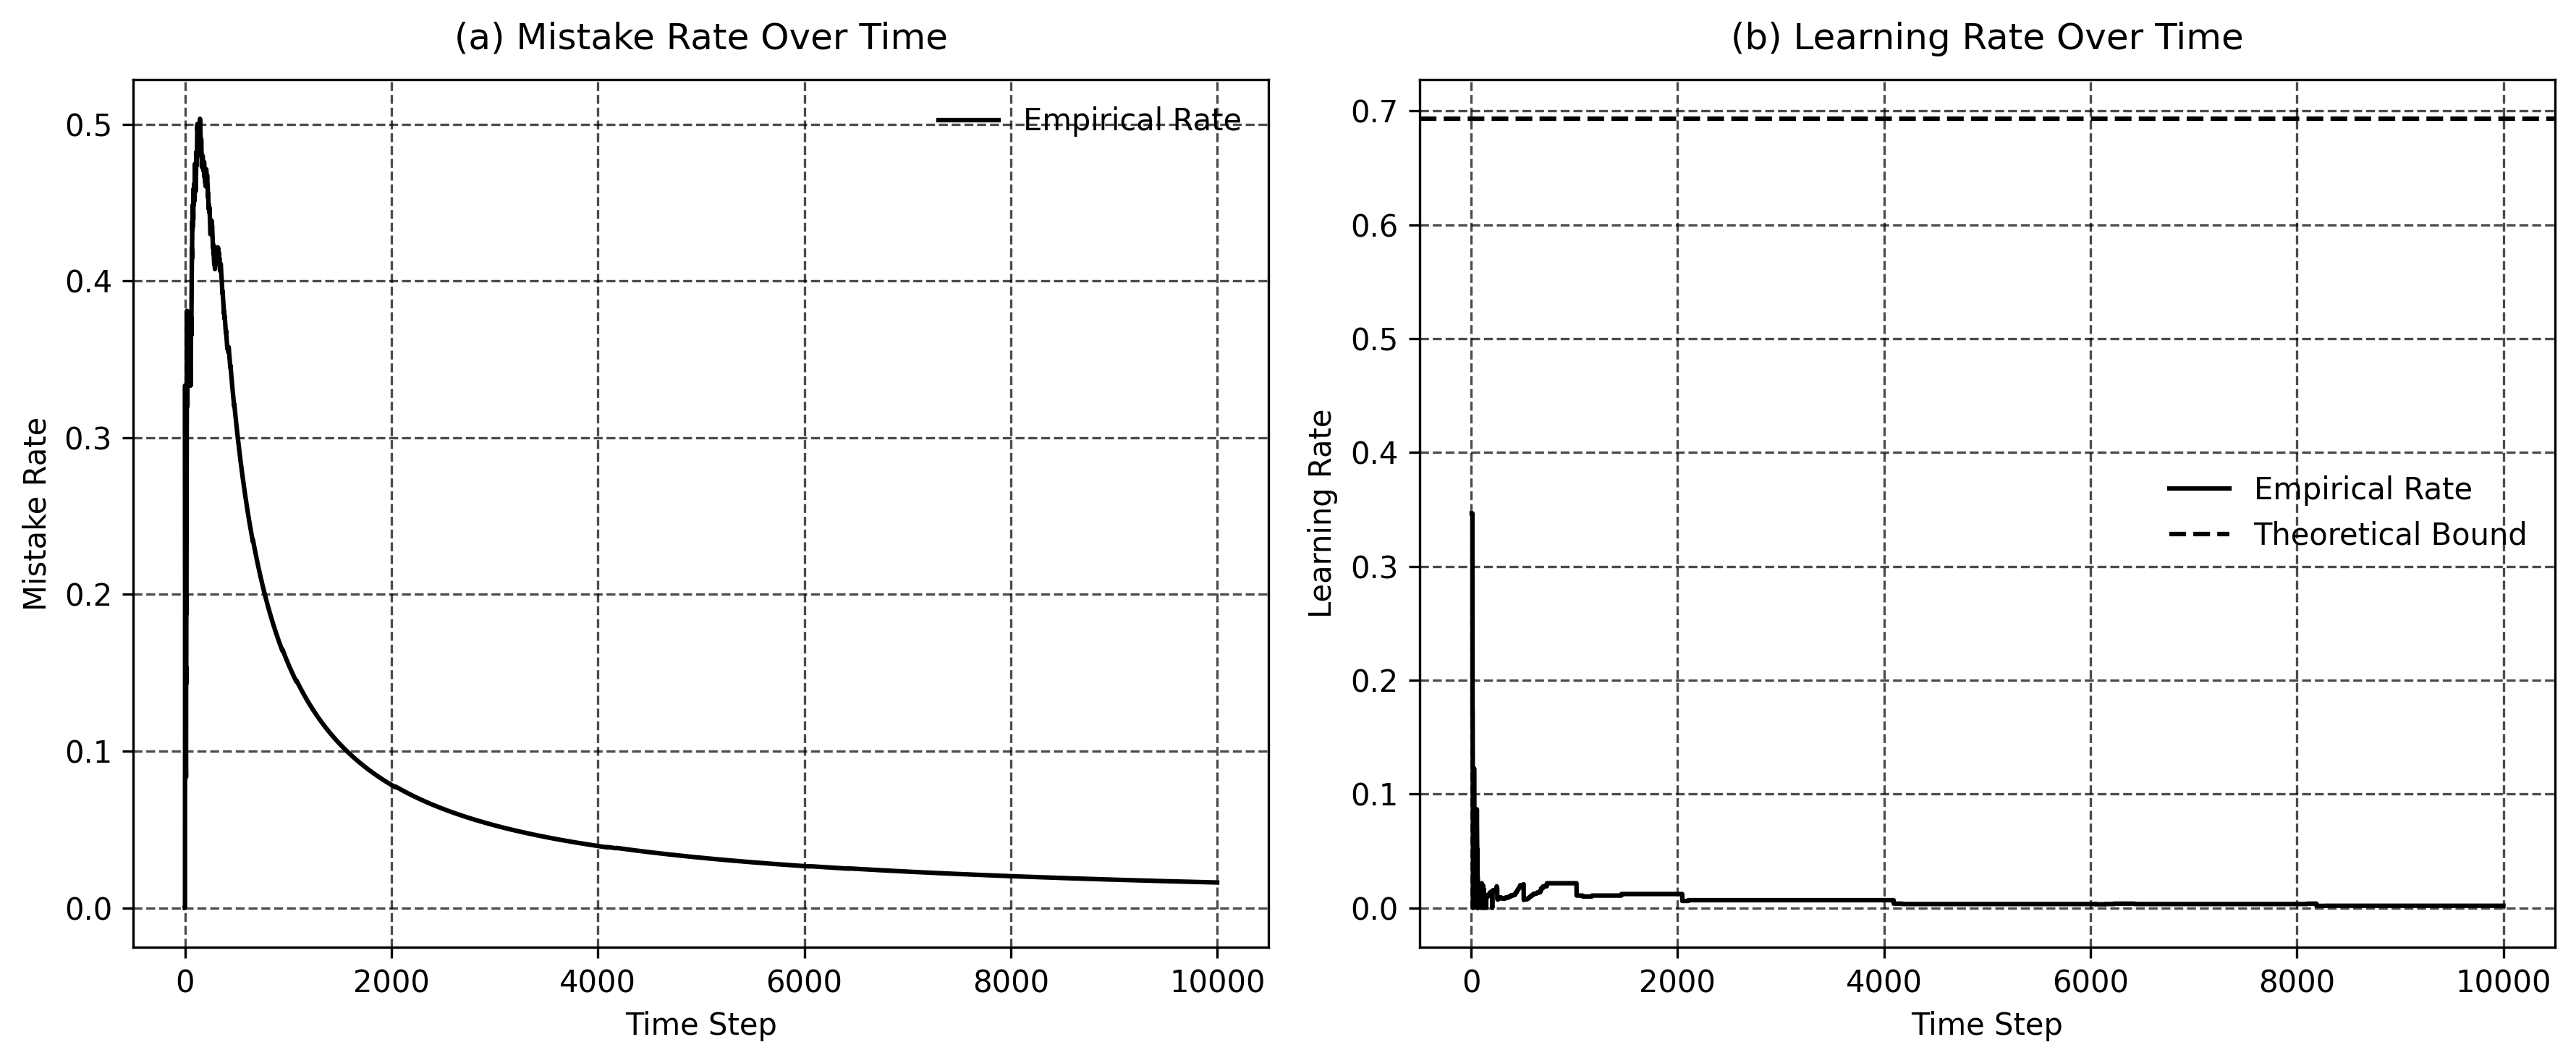
\includegraphics[width=1\textwidth]{../charts/single_agent_learning_curves_q=0.75.png}
    \caption{Learning curves for single agent}
    \label{fig:single-learning-curves}
\end{figure}

\subsection*{Multi-Agent Learning}

We extend our single-agent learning to a multi-agent setting using two different training paradigms: Centralized Training with Decentralized Execution (CTDE) and fully Decentralized Training with Decentralized Execution (DTDE). Both approaches maintain the core RNN architecture for processing observation histories while differing in their training mechanisms and information sharing structures. There are several aspects where they differ from the single-agent case. First, the GRU networks process not only individual signals but also the complete action profile. Second, we need to maintain individual networks to allow for decentralization. Finally, the learning dynamics in the multi-agent setting are influenced by the strategic interactions between agents, leading to non-stationarity in the environment.

\subsubsection*{Centralized Training with Decentralized Execution (CTDE)}

The CTDE approach employs a centralized critic during the training phase while maintaining decentralized actors for execution. This architecture enables information sharing during learning while preserving the decentralized nature of the deployed policies. The centralized critic has access to the global state and all agents' information during training, allowing it to better estimate the value of joint actions, while each agent's policy remains independent during execution.

\paragraph{Architecture Components}
\begin{itemize}
    \item \textit{Decentralized Actor Networks}: Each agent $i \in N$ maintains an independent actor network that maps their hidden state to a policy over actions:
    \[
        \pi^i_{\phi_i}(a^i_t|h^i_t) = \text{softmax}(W^i_{\pi}h^i_t + b^i_{\pi})
    \]
    where $\phi_i$ are the actor network parameters, $h^i_t$ is the agent's hidden state, and $W^i_{\pi}, b^i_{\pi}$ are the policy network weights and biases.
    
    \item \textit{Centralized Critic Network}: A single critic network processes the augmented state which includes the true state, signals, actions, and hidden states of all agents:
    \begin{align*}
        Q_{\xi}(\tilde{\psi}_t) &= W_Q f_Q(\tilde{\psi}_t, \mathbf{h}_t) + b_Q \\
        \mathbf{h}_t &= (h^1_t, \ldots, h^n_t)
    \end{align*}
    where $\xi$ are the critic network parameters, $\tilde{\psi}_t = (\omega, (s^i_t)_{i \in N}, \mathbf{a}_t, \mathbf{h}_t)$ is the augmented state, and $f_Q$ is a neural network that processes the joint input.
\end{itemize}

\paragraph{Training Process}
The CTDE training process operates by alternating between the following updates:

\begin{enumerate}
    \item \textit{Centralized Critic Update}: The critic is trained to minimize the temporal difference error across all agents:
    \[
        \mathcal{L}(\xi) = \mathbb{E}\left[(r_t + \gamma Q_{\xi}(\tilde{\psi}_{t+1}) - Q_{\xi}(\tilde{\psi}_t))^2\right]
    \]
    where $r_t$ is the immediate reward, and $\gamma$ is the discount factor.
    
    \item \textit{Decentralized Actor Updates}: Each actor network is updated using the policy gradient theorem with advantages computed by the centralized critic:
    \[
        \nabla_{\phi_i} J(\phi_i) = \mathbb{E}\left[\nabla_{\phi_i} \log \pi^i_{\phi_i}(a^i_t|h^i_t) A^i(\tilde{\psi}_t)\right]
    \]
    The advantage function $A^i(\tilde{\psi}_t)$ for each agent is computed as:
    \[
        A^i(\tilde{\psi}_t) = Q_{\xi}(\tilde{\psi}_t) - V_{\xi}(\tilde{\psi}_t)
    \]
    where the value function $V_{\xi}$ is computed by taking expectation over all agents' actions:
    \[
        V_{\xi}(\tilde{\psi}_t) = \mathbb{E}_{\mathbf{a}_t \sim \prod_{i \in N}\pi^i_{\phi_i}}[Q_{\xi}(\tilde{\psi}_t)]
    \]
\end{enumerate}

This training scheme allows each agent to benefit from global information during learning while maintaining the ability to act based solely on local observations during execution, analogous to a social planner. The centralized critic helps address the non-stationarity problem in multi-agent learning by incorporating the policies of all agents into its value estimation, while the decentralized actors ensure that the final policies remain executable with only local information.

\subsubsection*{Decentralized Training with Decentralized Execution (DTDE)}

The DTDE approach implements complete decentralization during both training and execution phases. Each agent learns independently using only their local observations and individual reward signals, without access to a centralized critic or global state information. This fully decentralized architecture ensures that agents can learn and operate autonomously, making it particularly suitable for settings where centralized training is impractical or undesirable.

\paragraph{Architecture Components}
\begin{itemize}
    \item \textit{Independent Actor-Critic Pairs}: Each agent $i \in N$ maintains both an actor network for policy learning and a critic network for value estimation:
    \begin{align*}
        \pi^i_{\phi_i}(a^i_t|h^i_t) &= \text{softmax}(W^i_{\pi}h^i_t + b^i_{\pi}) \\
        V^i_{\xi_i}(h^i_t) &= W^i_v f_v(h^i_t) + b^i_v
    \end{align*}
    where $\phi_i$ and $\xi_i$ are the actor and critic network parameters respectively, $h^i_t$ is the agent's hidden state, and $f_v$ is a neural network processing the hidden state.
    
    \item \textit{Local Value Estimation}: Each agent's critic estimates the expected discounted sum of future rewards based solely on their local information:
    \[
        V^i_{\xi_i}(h^i_t) = \mathbb{E}_{\pi^i}\left[\sum_{k=0}^{\infty} \gamma^k r_{t+k}^i \mid h^i_t\right]
    \]
    where $r_{t+k}^i$ represents agent $i$'s reward at time $t+k$, and the expectation is taken with respect to the agent's own policy $\pi^i$.
\end{itemize}

\paragraph{Training Process}
Each agent $i \in N$ trains independently through the following updates:

\begin{itemize}
    \item \textit{Local Critic Updates}: The critic network parameters $\xi_i$ are updated to minimize the temporal difference error:
    \[
        \mathcal{L}(\xi_i) = \mathbb{E}\left[(r_t^i + \gamma V^i_{\xi_i}(h_{t+1}^i) - V^i_{\xi_i}(h_t^i))^2\right]
    \]
    where $r_t^i$ is the immediate reward received by agent $i$.
    
    \item \textit{Local Actor Updates}: The actor network parameters $\phi_i$ are updated using policy gradient with locally computed advantages:
    \[
        \nabla_{\phi_i} J(\phi_i) = \mathbb{E}\left[\nabla_{\phi_i} \log \pi^i_{\phi_i}(a^i_t|h^i_t) A^i(h^i_t)\right]
    \]
    The advantage function $A^i(h^i_t)$ is computed using the local critic's value estimates:
    \[
        A^i(h^i_t) = r_t^i + \gamma V^i_{\xi_i}(h_{t+1}^i) - V^i_{\xi_i}(h_t^i)
    \]
\end{itemize}

This fully decentralized approach is beneficial for scalability and robustness, as each agent can learn independently without the need for centralized coordination. However, the lack of information sharing during training may lead to slower convergence or suboptimal coordination compared to CTDE approaches, particularly in settings where cooperative behavior is essential for optimal performance.

\subsubsection*{Experimental Setup}
The implementation is evaluated over a single continuos training run for signal accuries of $q \in \{0.1, 0.9\}$ to test the robustness of learning across informativeness of the signal for both paradigms with $T=10^5$ steps each. We track the evolution of the mistake rate, policies and empirical learning rate over time to compare against the theoretical bound. The results are visualized in Figure \ref{fig:multi-learning-curves-ctde} and \ref{fig:multi-learning-curves-dtde}. The learning curves demonstrate that the agent successfully learns to minimize mistakes and that the learning rate stays below the theoretical learning rate bound, validating the implementation.

\begin{figure}[htbp]
    \centering
    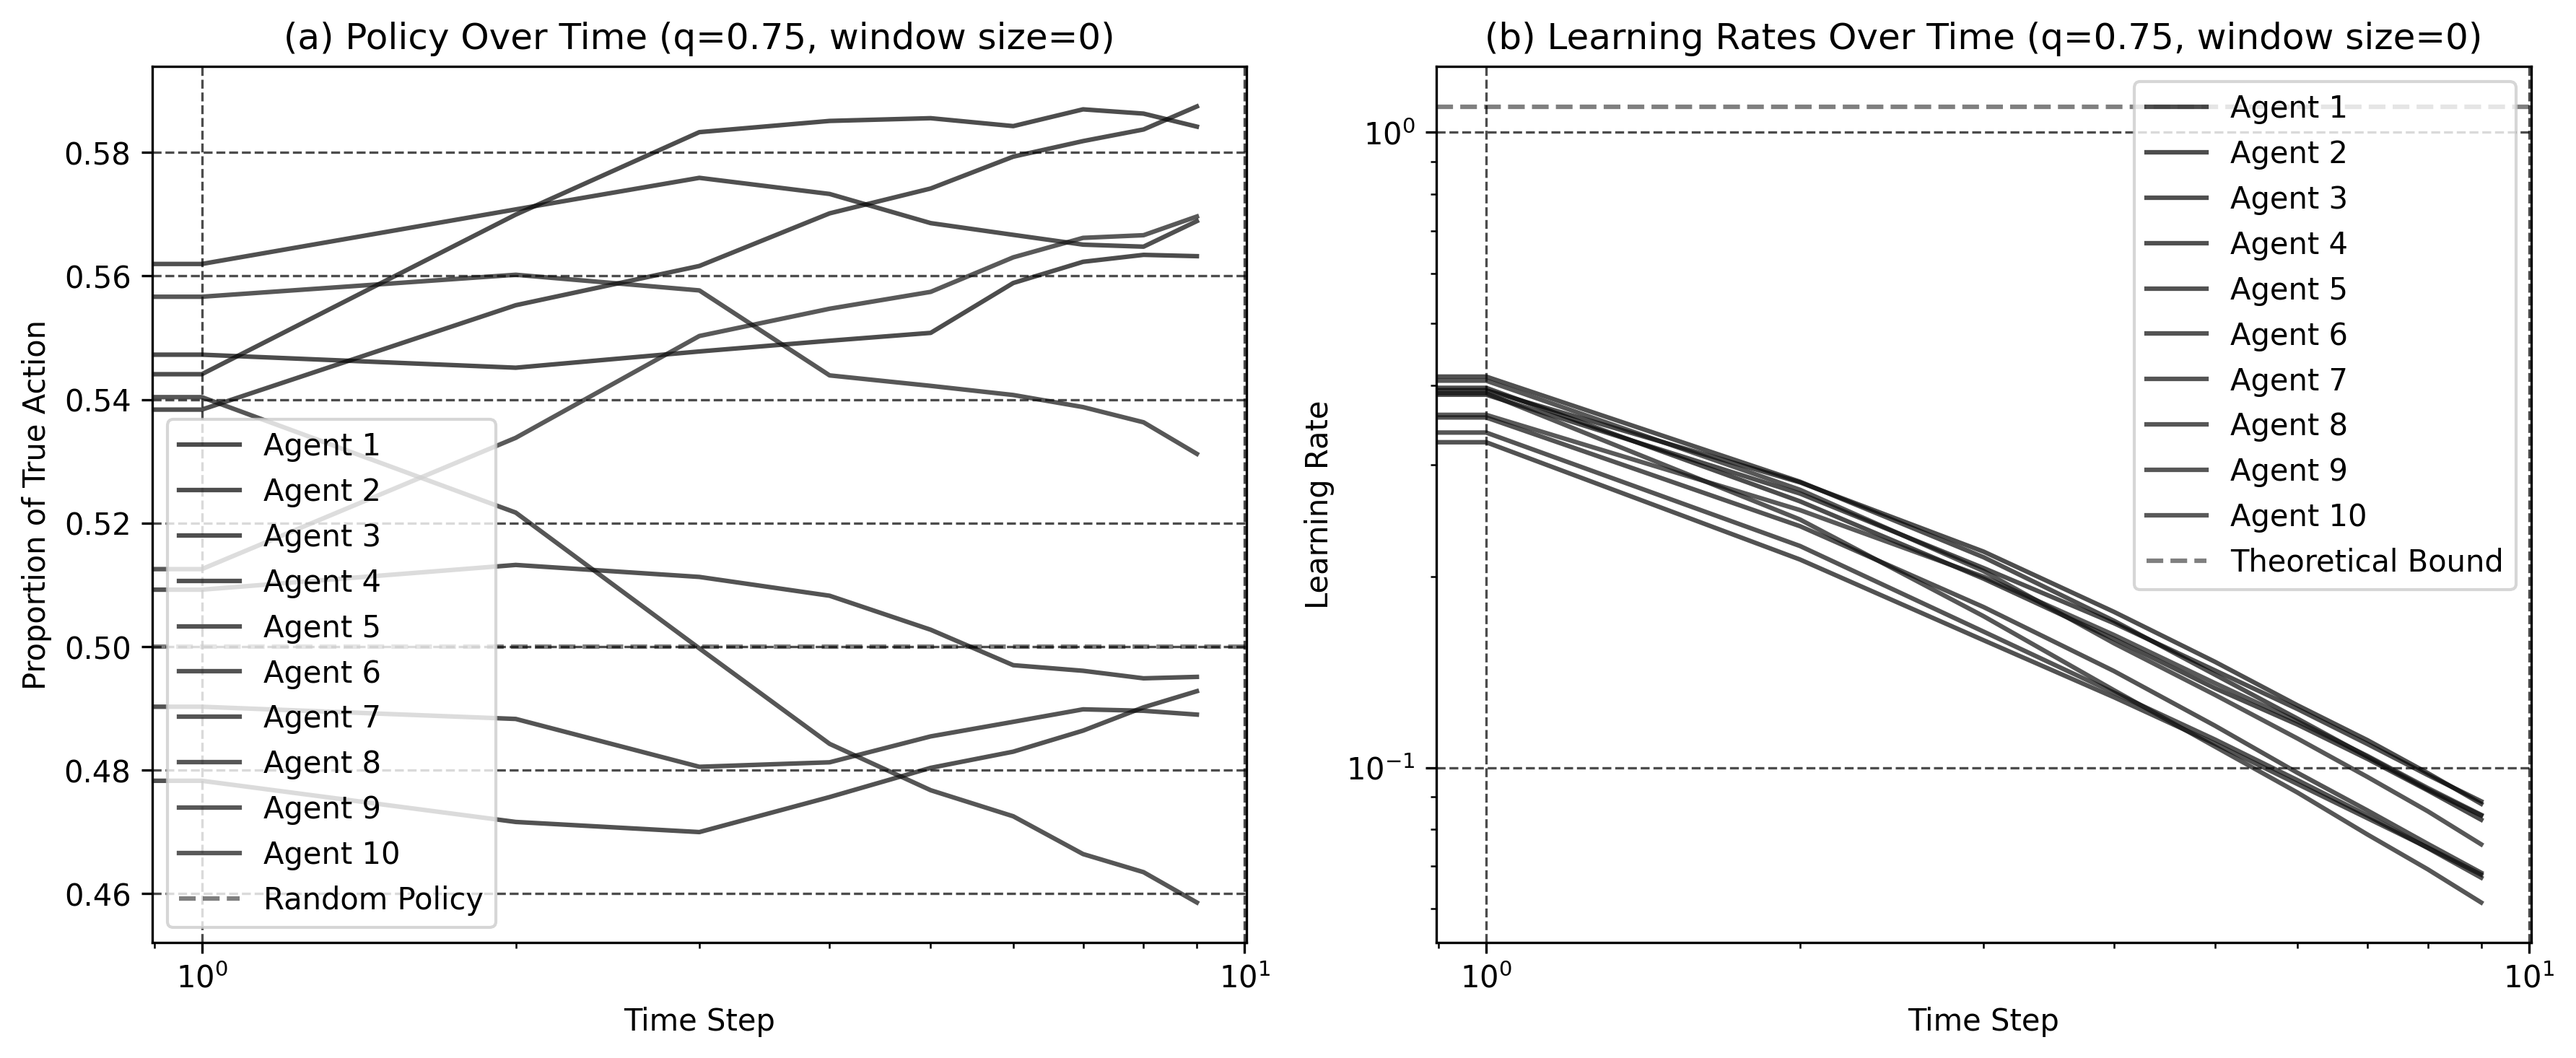
\includegraphics[width=1\textwidth]{../charts/multi_agent_ctde_learning_curves_q=0.75.png}
    \caption{Learning curves for multi-agent CTDE paradigm} 
    \label{fig:multi-learning-curves-ctde}
\end{figure}

\begin{figure}[htbp]
    \centering
    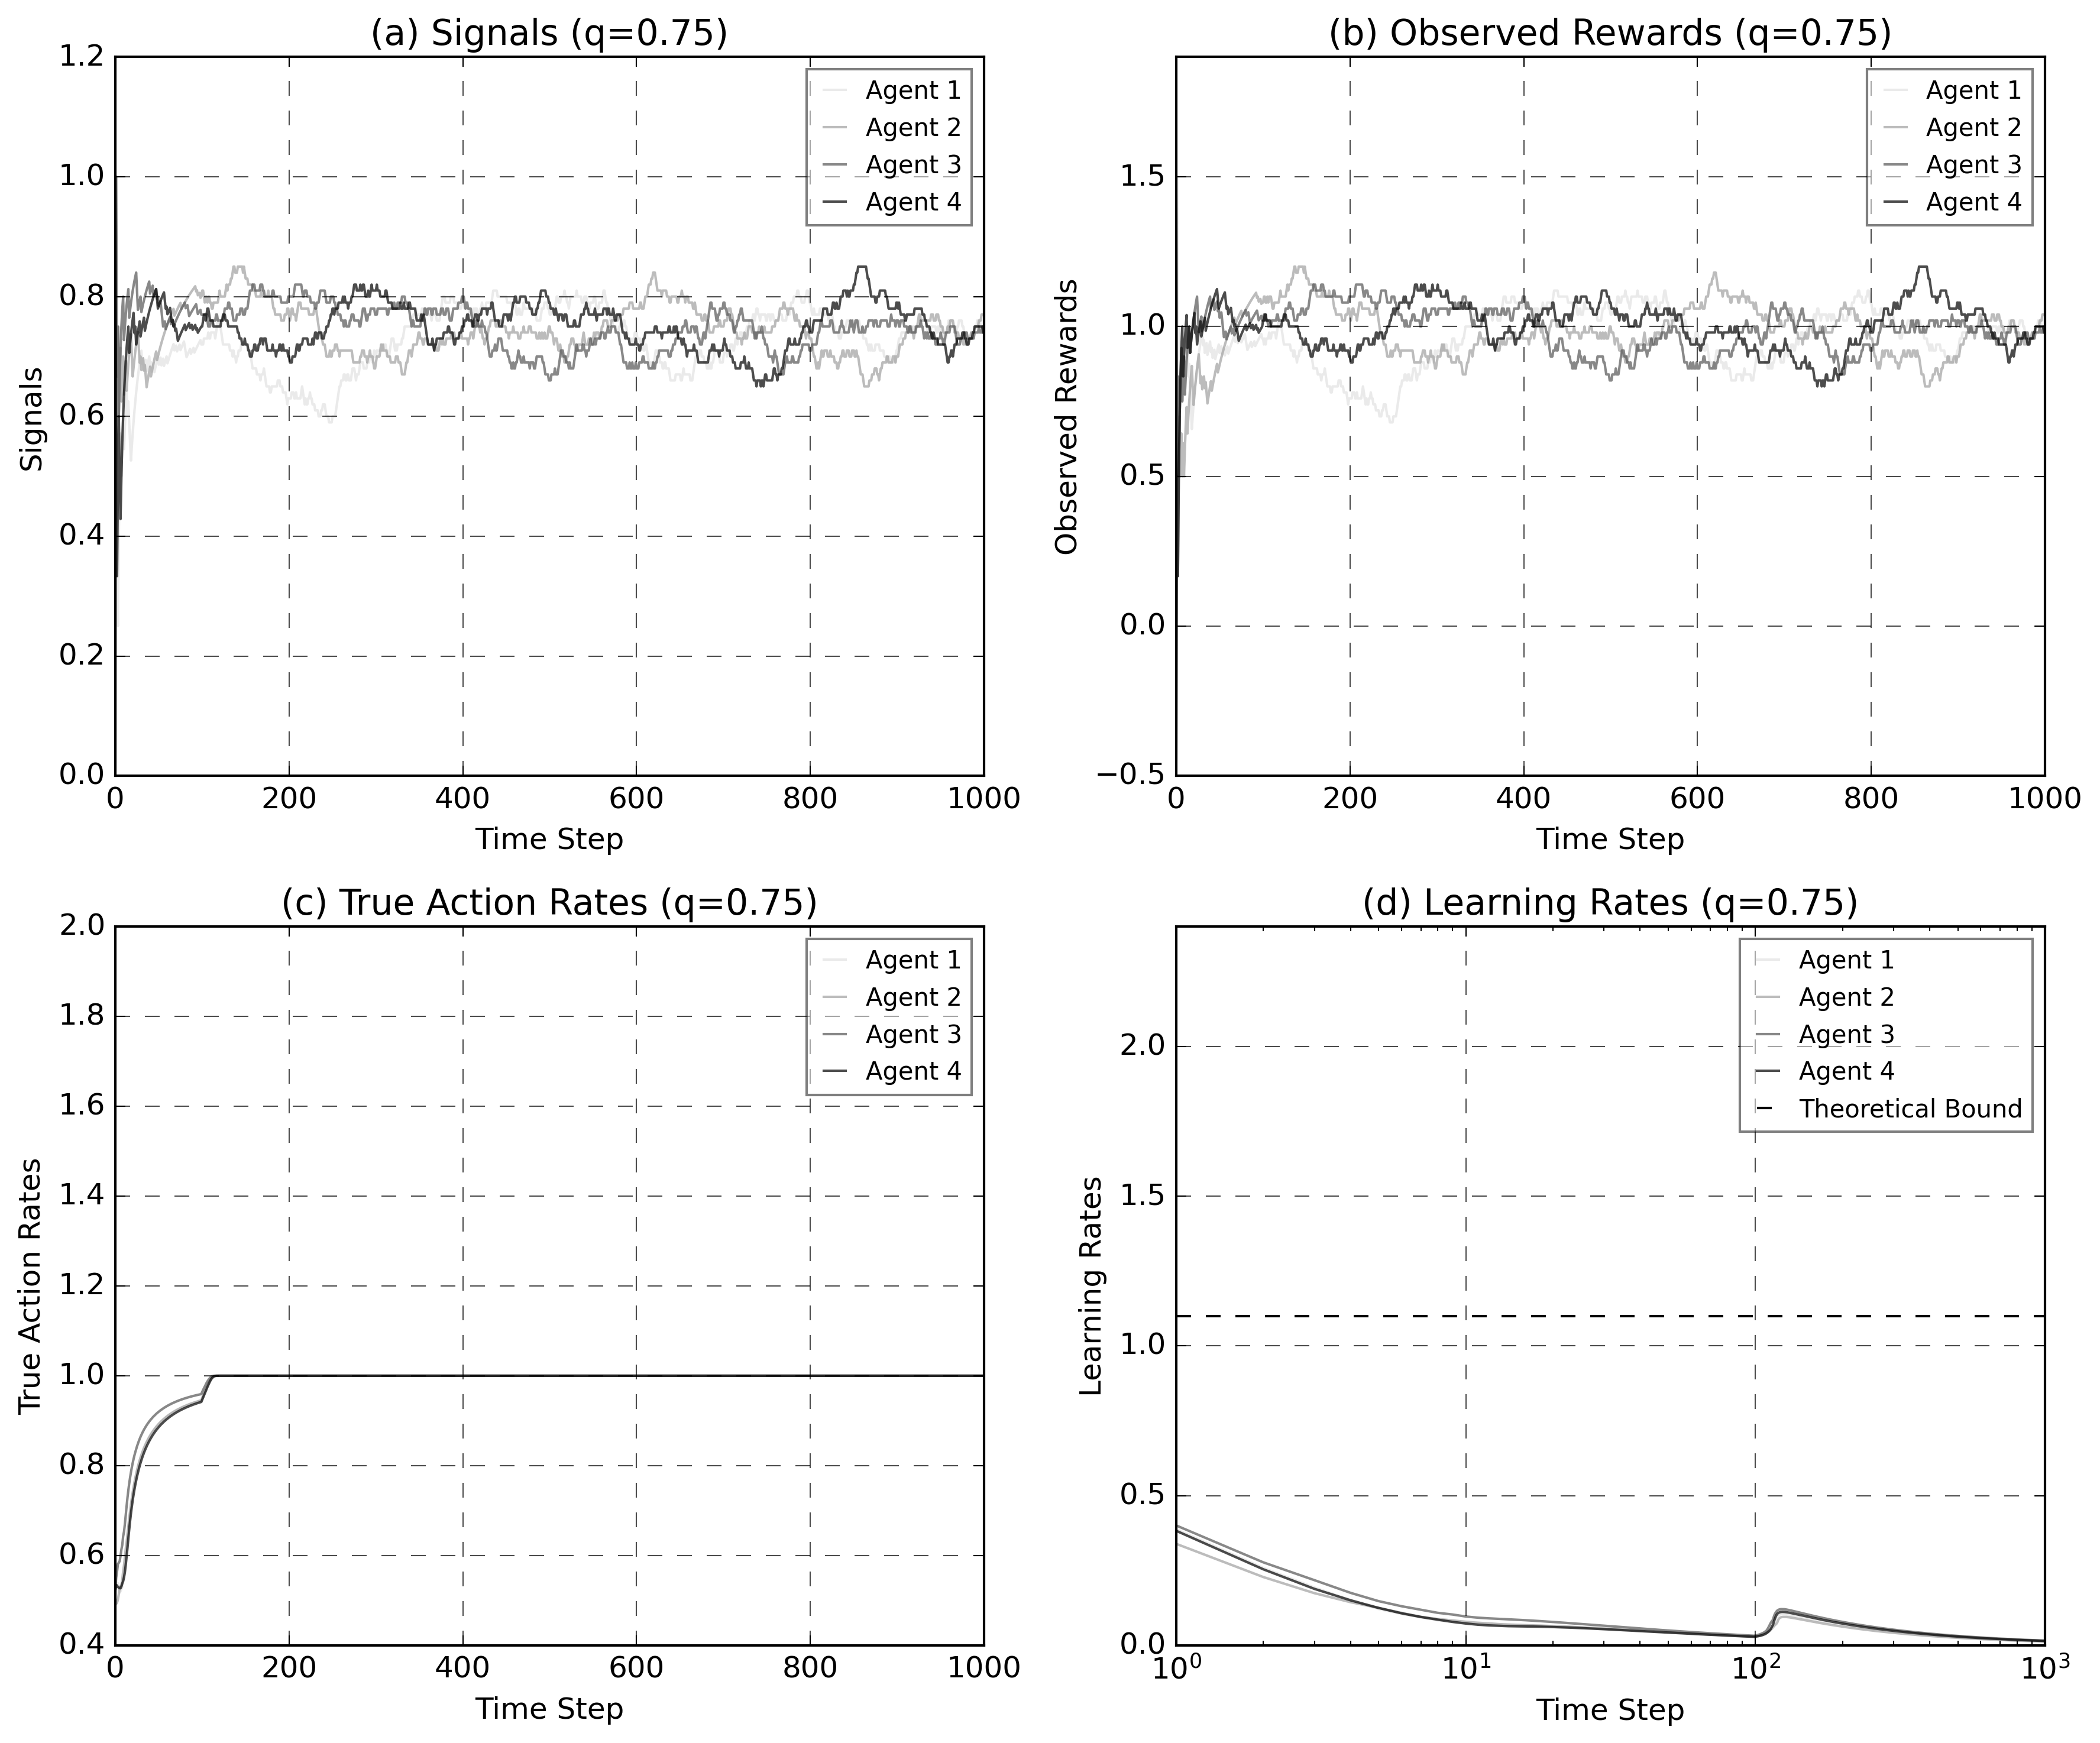
\includegraphics[width=1\textwidth]{../charts/multi_agent_dtde_learning_curves_q=0.75.png}
    \caption{Learning curves for multi-agent DTDE paradigm} 
    \label{fig:multi-learning-curves-dtde}
\end{figure}

\pagebreak